% Capítulo 6 (Resultados) — Slide 5 — Dispersão de CTI por política (figura isolada)
\begin{frame}{Dispersão de CTI por política}
  \centering
  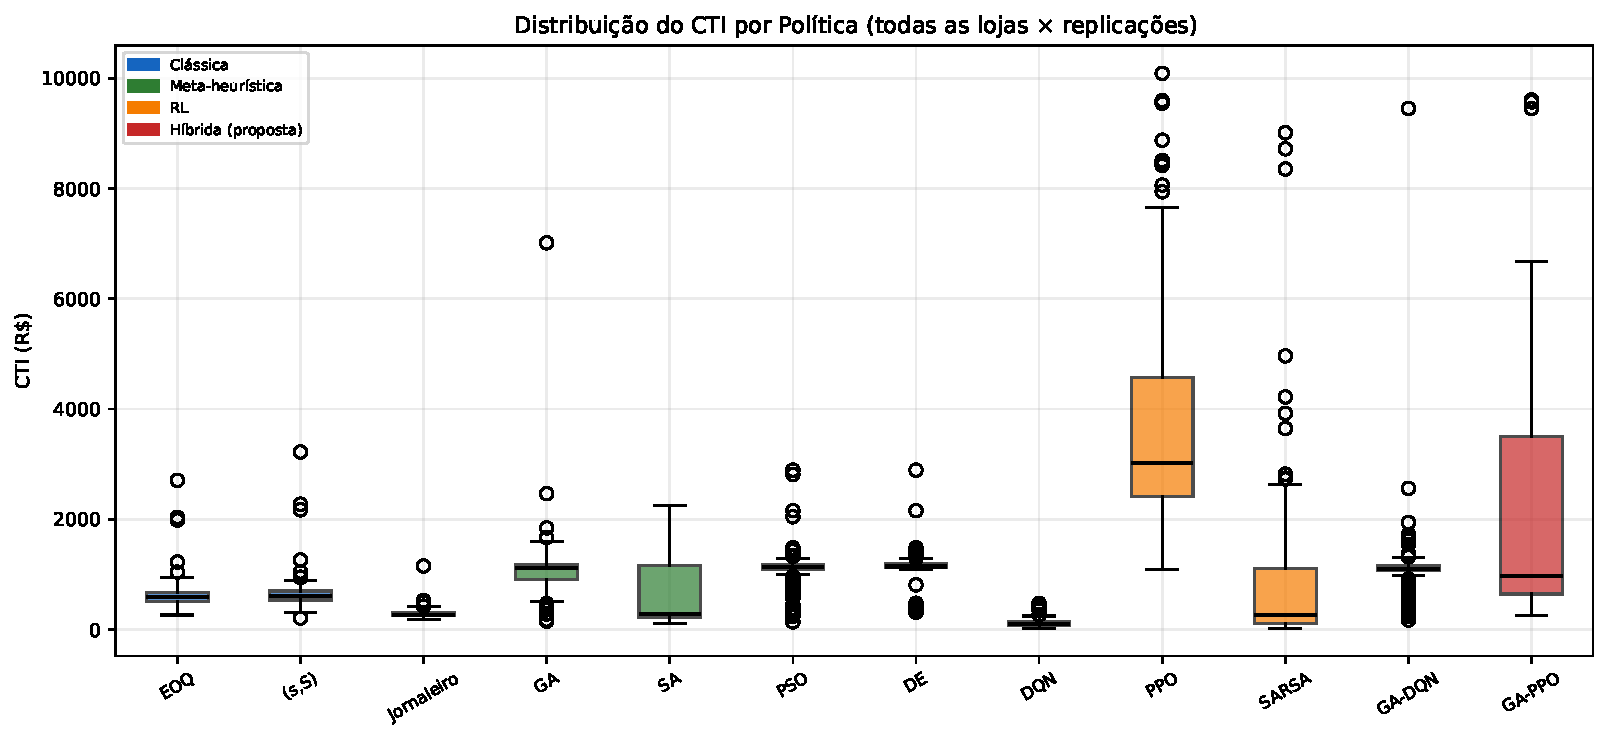
\includegraphics[width=0.62\linewidth,height=6.6cm,keepaspectratio]{figures/boxplot_tic.pdf}\\[0.4em]
  {\small Distribuição do CTI por política (boxplot sobre as 145 séries).}
  \note{
    Este boxplot mostra a distribuição de CTI de cada política sobre as 145
    séries. Caixas mais altas indicam que a mesma política produz custos
    muito diferentes entre séries -- a eficácia depende do perfil da
    demanda, não apenas da política escolhida. Algumas políticas, como GA,
    GA-DQN e GA-PPO, têm coeficiente de variação de CTI acima de 100\% entre
    séries. Essa heterogeneidade dentro de cada política é, junto com a
    fronteira de Pareto do slide anterior, a evidência empírica central que
    sustenta a proposta do AIPE.
  }
\end{frame}
